\documentclass[10pt]{article}
\usepackage[a4paper,margin=0.75in,headheight=15pt]{geometry}
\usepackage[T1]{fontenc}\usepackage[utf8]{inputenc}
\usepackage{lmodern,microtype,amsmath,amssymb,graphicx,booktabs,xcolor,hyperref,fancyhdr,caption}
\definecolor{ink}{HTML}{152E3C}\definecolor{blue}{HTML}{0072B2}\definecolor{mint}{HTML}{009E73}\definecolor{orange}{HTML}{D55E00}
\hypersetup{colorlinks=true,linkcolor=blue,urlcolor=blue,pdftitle={Better Than Stockfish: Relaxfish},pdfauthor={Michael Emanuel Glover}}
\urlstyle{same}\setlength{\emergencystretch}{3em}
\pagestyle{fancy}\fancyhf{}\fancyhead[L]{\small\textcolor{ink}{RELAXFISH | RESEARCH ARTICLE}}
\fancyhead[R]{\small Glover | 2026}\fancyfoot[C]{\small\thepage}
\renewcommand{\headrulewidth}{0.4pt}\setlength{\parindent}{0pt}\setlength{\parskip}{8pt}
\captionsetup{font=small,labelfont=bf,justification=raggedright,singlelinecheck=false}
\begin{document}
\begin{center}
{\fontsize{29}{33}\selectfont\bfseries\color{ink} Better Than Stockfish:\\Relaxfish}\par\vspace{9pt}
{\large\color{blue}Hierarchical relaxation, adversarial evidence\\and empirical approximate solving}\par\vspace{9pt}
Michael Emanuel Glover\par
{\small Research article and extended methods | 3 October 2026}
\end{center}

\section*{Abstract and central proposition}
Chess is a finite adversarial system with an exact outcome and an immense space of possible explanations. I propose Relaxfish: a hierarchical relaxation architecture that represents pieces as interacting tactical agents, converts their coordinated roles into search priorities, and evaluates progress through adversarial testing and explicit uncertainty bounds. The ambition is straightforward: build an engine better than Stockfish, then investigate whether its strongest mutually adversarial policies support an empirical approximate solution of chess. That ambition deserves mathematics, executable experiments and a demanding opponent population. Here I provide all three at prototype scale. A seven-role field combines unary affinities, pairwise coalitions and genuine three-piece attack terms. A simplex-preserving update increases a specified compatibility potential, while a separate exact solver propagates sound win/draw/loss intervals for a bounded multi-king habitat. In an executed 24-position diagnostic, role relaxation raises exact agreement with a 20,000-node Stockfish 14.1 reference from 6 to 10 positions and reduces the median signed diagnostic gap from 54 to 2.5 centipawns. Four diagnostic matches expose the present search bottleneck: the one-ply prototype loses every game. These measurements establish an operative mechanism and a sharp next experiment. They do not establish superiority over current Stockfish. The article develops the stronger claim in operational terms: empirical solving requires specified opponent coverage, response-oracle quality, statistical confidence and a declared error tolerance. Exact certification requires sound strategic bounds. The central research programme is to make those bounds and that evidence converge.

\subsection*{A statement of intent}
Reality always has veto power. That is the governing principle of this work. I want a powerful claim to survive a powerful test. Better Than Stockfish'' names the target of the programme; the measurements identify where the current implementation stands. The title is deliberately ambitious, and the methods make the ambition accountable.

The governing question is whether a relational account of a position can improve the allocation of computation enough to produce stronger play and more informative certificates. A rook is material, geometry and an agent in a plan. A pawn can be a runner, a shield, an obstruction or the hinge of a mating net. Those descriptions interact. Relaxfish treats that interaction as computable structure rather than decorative narration.

\clearpage
\section*{1. The problem is larger than a leaderboard}
A match score answers a practical question: which tested programme performs better under specified conditions? A solution asks a strategic question: what can each side guarantee against every admissible opponent? Both questions are valuable. Their relationship becomes precise only when the opponent class, resource budget and game rules are written down.

I reject the idea that empirical evidence becomes uninteresting merely because it is not a universal proof. Modern computational research advances by testing increasingly demanding models against increasingly demanding counterexamples. An engine that withstands a diverse adversarial league has achieved something real. The right task is to describe the scope of that achievement, quantify its uncertainty and deliberately enlarge the set of attacks against it.

The game-theoretic value is not a popularity contest among evaluators. Agreement between powerful engines can reflect convergence toward the same underlying strategy, shared training information, similar search biases or a common blind spot. Relaxfish therefore makes diversity a property of the experiment. Architectural differences, budget escalation, opening perturbations, tactical counterexamples and response-oracle searches enter the evaluation explicitly.

There are two linked engines in this article. The standard-board prototype implements relational evaluation and one-ply choice using python-chess. The habitat solver implements exact integer bounds for Chess Critter, a separate rectangular multi-king variant. Their present separation is useful: one develops strategic representations; the other makes the semantics of certification visible. Merging them is a future implementation task, not a completed experimental result.

The proposition is that relational inference can become an efficient interface between local geometry and global adversarial reasoning. That proposition has a clear failure condition. If role inference consumes computation without improving strength at equal wall time, its explanatory appeal is insufficient. If a representation concentrates probability but loses to a simple counterexample, its confidence is misplaced. A research programme earns its force by exposing those possibilities early.

\begin{minipage}{\linewidth}\begin{center}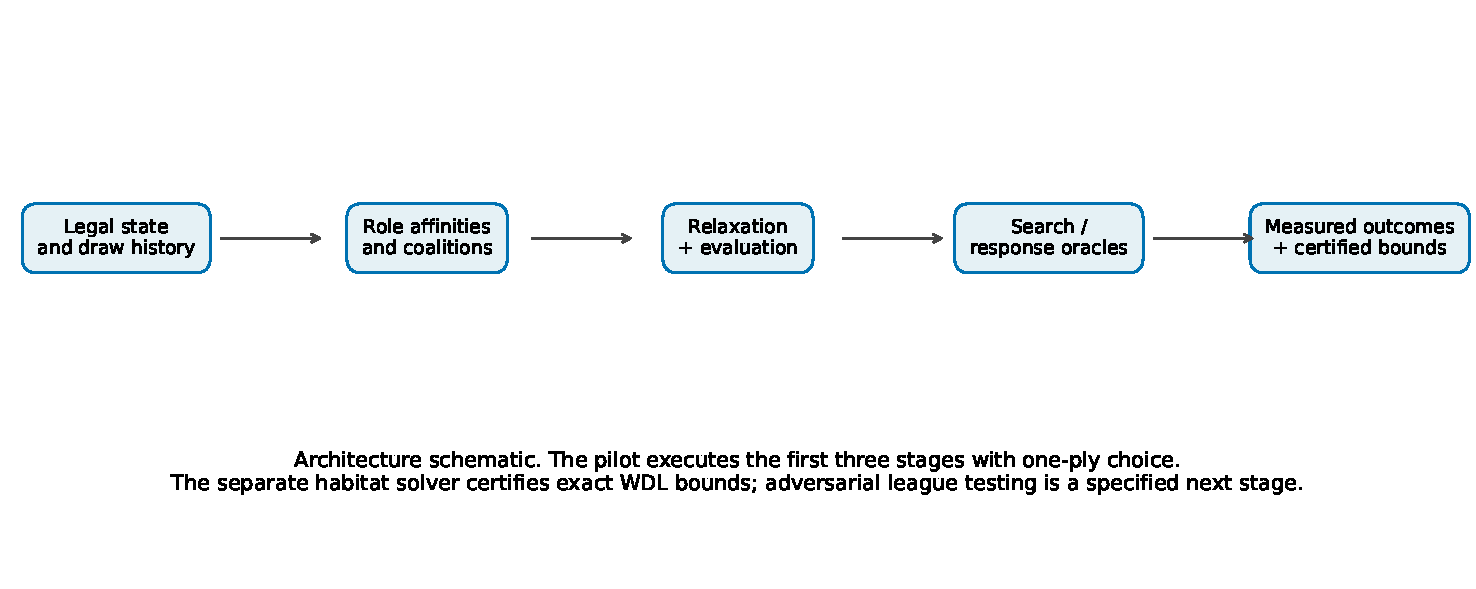
\includegraphics[width=.97\linewidth,height=.35\textheight,keepaspectratio]{figures/architecture.pdf}\end{center}
{\small\textcolor{ink}{Figure 1. Relaxfish architecture and implemented scope. Blue blocks identify the sequence from complete legal state to relational inference, search and evidence. The standard-board pilot executes role inference and one-ply evaluation. Exact habitat bounds are supplied by a separate solver. The response-oracle league is a specified next stage.}\par}\end{minipage}

\clearpage
\section*{2. Three meanings of a solution}
Let $\mathcal G$ be a completely specified two-player zero-sum game and let $s$ denote a state. White receives utility $u\in\{-1,0,+1\}$ for a Black win, draw or White win. For possibly randomized policies $\pi_W$ and $\pi_B$, define $u_s(\pi_W,\pi_B)$ as expected terminal utility. The starting-state value is

\[
V^*(s)=\sup_{\pi_W}\inf_{\pi_B}u_s(\pi_W,\pi_B).
\]

For a finite perfect-information game with deterministic rules, backward induction supplies the corresponding minimax value. The practical challenge is the size of the state space, not the existence of the definition. Rules involving repetition require history-sensitive state; a diagram alone is not always sufficient.

I distinguish three claims. A benchmark superiority claim states that one engine wins under a named testing protocol. An empirical approximate-solving claim states that tested strategies resist the specified response class within a declared tolerance and confidence level. An exact-solving claim identifies the game-theoretic value through a valid strategic certificate. These claims form a research ladder, not a ranking of which evidence matters.

The paper's title belongs to the first target. Its formal development connects the second target to the third. A programme can outperform the reference engine before it can certify an opening. It can certify selected endings while remaining weaker in practical play. Conversely, repeated draws between its own policies can be informative without settling whether an untested strategy forces a win.

The value is always indexed by the game. Official chess, a game with automatic claimable draws, a fixed-ply truncation and a multi-king habitat need not have the same value. The common language of win, draw and loss does not erase these differences. Each conclusion in this article carries the rule system under which it is valid.

That discipline increases the reach of the programme. It permits exact statements about tractable variants, diagnostic statements about a prototype, and substantial empirical statements about a future league without forcing them into one inappropriate notion of proof.

\clearpage
\section*{3. Epsilon has a job to do}
An error tolerance is useful when it measures a defined quantity. Relaxfish uses separate symbols for strategic uncertainty, sampling uncertainty and numerical error. The separation is operational: each quantity has a different source, a different estimator and a different remedy.

For candidate policies, define the guarantees and threats

\[
L(\pi_W)=\inf_{\pi_B}u_s(\pi_W,\pi_B),\qquad
U(\pi_B)=\sup_{\pi_W}u_s(\pi_W,\pi_B).
\]

They bracket the value: $L(\pi_W)\le V^*(s)\le U(\pi_B)$. The policy-pair gap $g=U-L$ measures the unresolved strategic interval. If both endpoints are close to zero, the evidence is close to a draw in the game-theoretic sense. A small gap somewhere else can identify a near-optimal winning or losing position instead.

For randomized policies, a guarantee may lie between the three terminal values. Consequently, a small exploitability gap alone does not automatically identify the exact discrete value. The exact conclusion requires an interval containing only one member of $\{-1,0,+1\}$. In particular, certified guarantees $L> -1$ and $U<+1$ identify a draw for the underlying deterministic finite game. This condition refers to universal bounds, not merely the average outcome of self-play.

Sampling uncertainty concerns the estimate of performance against a declared distribution of challenges. Numerical error concerns arithmetic and implementation. A standard deviation of centipawn scores, a confidence interval for a match mean and a tolerance of $10^{-64}$ on a floating-point residual do not become interchangeable because all are small numbers.

My original intuition was to make epsilon tiny. The sharper version is to make it meaningful first. A useful error ledger is

\[
\epsilon_{\rm declared}=\epsilon_{\rm statistical}+
\epsilon_{\rm oracle}+\epsilon_{\rm coverage}+\epsilon_{\rm numerical},
\]

provided all four terms bound the same utility-scale target and their assumptions justify addition. A term without an upper bound remains unresolved; it cannot be assigned zero by enthusiasm. This is how an ambitious empirical claim acquires a mathematical spine.

\clearpage
\section*{4. A hierarchy of tactical agents}
Classical material values summarize exchange potential. They leave considerable structure implicit. Two rooks can contest the same file, a bishop can guard the route of a passer, and three attackers can restrict a king more effectively than three isolated threats. Relaxfish assigns each live piece a distribution over roles and updates those distributions through their relationships.

The role alphabet is $\mathcal R=\{A,D,C,O,R,T,I\}$: attacker, defender, controller, outpost, runner, tactician and idle. For piece $i$, $q_i\in\Delta^6$ contains nonnegative weights summing to one. These weights express relative role support. They are not calibrated probabilities of winning or proof that a plan works.

The hierarchy has four levels. Board geometry supplies legal moves, attacks and king zones. Individual affinities connect that geometry to roles. Pairwise coalitions express cooperation between roles. Three-piece factors express attack clusters that cannot be represented by counting each attacker independently. Search then tests the consequences of the representation against the opponent's responses.

The visual identities come from the definitive Woodland cast in Maestro. King Ethelheim and Queen Dilorias inhabit the same mathematical roles as a conventional king and queen. Their names do not change legal movement or material accounting. The distinction matters because an interpretable interface should reveal the model's state without smuggling a different game into the comparison.

The current prototype reimplements the relational idea in a compact Python experiment. It is not a byte-for-byte translation of the browser labeler. The browser's signed coalition terms and minimum-subtraction normalization are replaced by a symmetric compatibility construction and an explicitly monitored objective. The change makes the implemented update easier to inspect and differentiate.

Role language has practical value only if it changes computation in useful ways. The pilot asks whether it changes selected moves. The decisive future test asks whether those changes improve match performance at equal resource budgets. Narrative intelligibility and adversarial strength are complementary measurements; neither substitutes for the other.

\clearpage
\section*{5. The compatibility potential}
Let $a_{ir}\ge0$ be the unary affinity of piece $i$ for role $r$. Let $W=W^\top$ contain same-team relational weights, with zero diagonal. Let $C=C^\top$ describe role compatibility. Let $\mathcal T$ contain triples of distinct allied pieces attacking the opposing king zone. Define

\[
F(q)=\sum_{i,r}a_{ir}q_{ir}
+\frac{\lambda_2}{2N}\sum_{i,j,r,t}W_{ij}C_{rt}q_{ir}q_{jt}
+\frac{\lambda_3}{\max(1,|\mathcal T|)}
\sum_{(i,j,k)\in\mathcal T}q_{iA}q_{jA}q_{kA}.
\]

The factors $N$ and $\max(1,|\mathcal T|)$ control the scale of relational support as population and motif counts change. They do not establish invariance across all board sizes; that stronger property would need its own test. The factor one-half removes double counting of symmetric pair terms.

The unary terms are fixed by the current position. Attack affinities count influence in the enemy king zone; defensive affinities count influence near the friendly king. Controllers receive sliding-piece activity, outposts receive advanced minor-piece placement beyond enemy pawn attacks, runners receive advancement and passer structure, and tactical affinity includes attacked enemy material. An idle role records low geometric activity. Every affinity receives a positive floor of 0.02.

The support is the analytic gradient $g_{ir}=\partial F/\partial q_{ir}$. The pair term contributes $(\lambda_2/N)(WqC)_{ir}$. Each triple contributes the product of the other two attacker weights to the relevant derivative. Genuine triples require three different piece indices and a single team; duplicating one attacker would instead introduce a different polynomial interaction.

The potential is a compatibility objective, not the chess value. Maximizing $F$ can yield a coherent but unsound attack. The evaluation layer and adversarial search must decide whether that coherence survives legal replies. This distinction lets us prove useful properties of the inference mechanism without declaring its output an oracle.

\clearpage
\section*{6. The relaxation update and its guarantee}
The pilot initializes $q_{ir}=a_{ir}/\sum_t a_{it}$. A simultaneous exponentiated update proposes

\[
q_{ir}^{+}=\frac{q_{ir}\exp(\eta g_{ir})}
{\sum_tq_{it}\exp(\eta g_{it})}.
\]

Subtracting the largest support in each row before exponentiation leaves this expression unchanged and improves numerical stability. The candidate step begins at $\eta=1$ and is halved if the measured potential decreases beyond a $10^{-12}$ arithmetic allowance. At most 24 candidates are examined; if none is accepted, the previous state is retained. Twelve outer iterations are executed in the pilot.

\textbf{Proposition 1: simplex preservation.} If each row begins with positive entries, finite supports and a positive finite step, every updated row is positive and sums to one in exact arithmetic. The numerator is positive and the denominator is its positive row sum. In floating-point arithmetic, normalization and finite-value checks remain necessary.

\textbf{Proposition 2: an ascent direction.} At $\eta=0$, the derivative of the potential along the update is

\[
\left.\frac{dF(q^+(\eta))}{d\eta}\right|_{0}
=\sum_i\left[\sum_rq_{ir}g_{ir}^2-
\left(\sum_rq_{ir}g_{ir}\right)^2\right]\ge0.
\]

The expression is a sum of weighted variances. If at least one variance is strictly positive, differentiability implies an increasing sufficiently small step exists. If all variances vanish, the update leaves each row unchanged. The implemented acceptance check therefore provides monitored nondecrease up to its stated arithmetic allowance. It does not establish convergence to a global maximum.

The guarantee is deliberately local to the object being optimized. Relaxation concentrates a representation; minimax evaluates a contest. A stationary role field can coexist with a losing move. A strong engine requires the representation to improve search efficiency and response quality, not merely to settle into a confident description.

The experiment records every potential and entropy trajectory. Numerical finite differences verify every gradient component on the Sicilian fixture, independently of the trajectory check. These are implementation checks on the relational mechanism, not chess-strength certificates.

\begin{minipage}{\linewidth}\begin{center}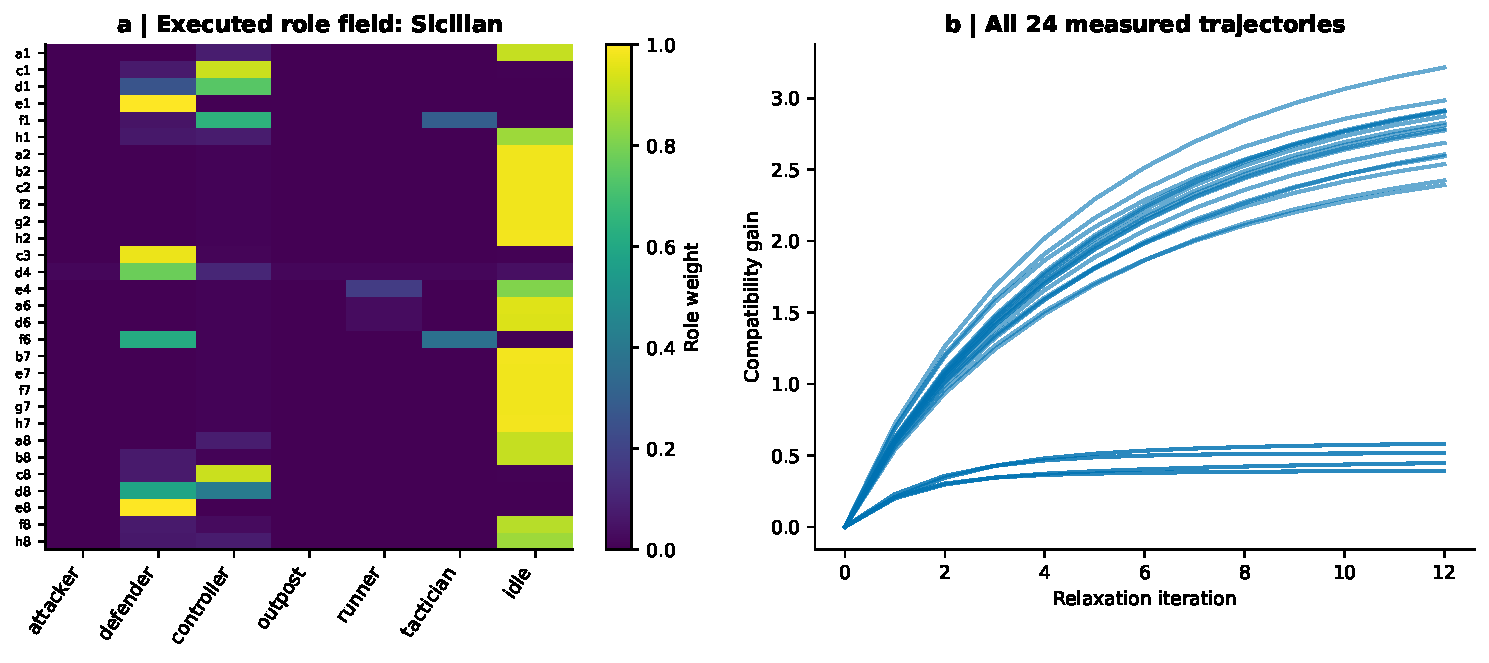
\includegraphics[width=.97\linewidth,height=.35\textheight,keepaspectratio]{figures/role_field.pdf}\end{center}
{\small\textcolor{ink}{Figure 2. Executed role inference. Left, the final seven-role distribution for every piece in the Sicilian fixture, with square identities on the vertical axis. Right, compatibility gain across twelve updates for all 24 fixtures. All trajectories come from the released computation; brighter role weights denote concentration rather than calibrated strategic certainty.}\par}\end{minipage}

\clearpage
\section*{7. From representation to a move}
The prototype's static evaluation uses material values of 100, 320, 330, 500 and 900 centipawns for pawn, knight, bishop, rook and queen. Kings receive no exchange value. Minor pieces receive a small centralization term, and pawns receive a directional advancement term. This deliberately simple evaluator creates a transparent ablation baseline.

The role contribution is

\[
E_{\rm role}(s)=18\sum_i\sigma_i\sum_rw_rq_{ir},\qquad
w=(0.8,0.7,0.45,0.55,0.9,1.0,-0.3),
\]

where $\sigma_i=+1$ for White and $-1$ for Black. The coefficients are manually specified pilot parameters. They were not fitted to the diagnostic outcomes, and the paper does not present them as optimal. The full nonterminal evaluation is $E(s)=E_{\rm static}(s)+E_{\rm role}(s)$.

At the root, all legal moves are visited in deterministic UCI order. The one-ply prototype evaluates their successor positions and selects the maximum for White or minimum for Black. Terminal outcomes receive utility-derived scores, with wins and losses mapped to $\pm100{,}000$ for the chooser and draws to zero. The baseline uses the identical chooser with the role term removed.

This design isolates the effect of relational evaluation at fixed search depth. It does not hold computational cost constant: role inference makes each leaf more expensive. Fixed-depth comparisons answer whether the representation changes decisions; fixed-time comparisons must answer whether it improves an engine.

The current chooser has no quiescence extension, transposition table, null-move pruning, trained value network or mature tactical search. Naming these absent components is useful because the diagnostic losses identify where development effort should go. A one-ply score can favor a capture whose recapture lies just beyond its horizon.

The intended production architecture uses the role field first for move ordering and attention allocation. Ordering retains all legal alternatives and can accelerate exact or conventional search without turning role confidence into a pruning certificate. Selective pruning is a separate, more demanding engineering decision. Its speed gains must be tested against tactical failure and any impact on sound bounds.

\clearpage
\section*{8. The executed diagnostic}
The released pilot contains 24 fixed positions: eight conventional opening positions, eight middlegames generated by deterministic uniformly sampled legal moves, and eight synthetic endings. The seed is 20261003. Each category contributes equally to the descriptive aggregate. This is an implementation diagnostic with a known construction, not a representative sample of tournament chess.

The opening fixtures span the Italian, Sicilian, French, Caro-Kann, Queen's Gambit, King's Indian, English and Reti. The legal-random middlegames intentionally expose irregular geometry. Their moves are sampled in sorted UCI order, and their requested lengths increase from 24 to 38 plies. All selected states pass python-chess validity checks and are nonterminal. The ending fixtures include mirrored king-and-queen, promotion, rook and blocked-pawn configurations.

Stockfish 14.1 is the locally installed comparator. It runs with one thread and a 16 MiB hash. The binary's SHA-256 digest and reported identity are stored with the data. A 20,000-node search supplies the reference move. A 2,000-node search supplies a lower-budget same-engine comparator. The hash is cleared before these analyses.

The diagnostic evaluates each selected move's successor with a separate 5,000-node Stockfish analysis from the original mover's perspective. Terminal successors are scored directly. Mate scores are mapped to a signed 10,000-centipawn surrogate for plotting and tabulation. This mapping is conventional instrumentation for this experiment; it is not a claim that mate has a finite exchange value.

All positions, moves, role fields, traces and evaluation gaps are released. Their labels do not imply hidden human annotations or curated tactical truth. Reference agreement tests concordance with a versioned evaluator. It does not prove optimality, and disagreement does not necessarily mean the alternative is inferior.

The prototype treats claimable draws as terminal automatically through outcome(claim\_draw=True), rather than modelling a player's optional draw claim. This is an explicit pilot convention and differs from the official claim procedure. The four match demonstrations use two opening positions with colours reversed. They are intentionally small and unequal in resources: one-ply Relaxfish faces Stockfish at 1,000 nodes per move. They expose operational weaknesses before any serious superiority trial is launched. No Elo estimate is computed from four games.

\clearpage
\section*{9. What the pilot actually found}
Role inference changed the selected move in 9 of 24 positions. Exact agreement with the 20,000-node reference increased from 6/24 for the static evaluator to 10/24 for Relaxfish. Stockfish at 2,000 nodes agreed in 16/24 cases. The role model therefore makes a measurable decision-level difference in this suite while remaining behind the same-engine comparator.

The median signed post-move reference gap was 54 centipawns for the static model, 2.5 for Relaxfish and zero for Stockfish at 2,000 nodes. Mean gaps were approximately 1,070.3, 1,006.6 and 11.5 centipawns, respectively. The means are strongly influenced by the mate-score surrogate and should not be read as ordinary positional centipawn losses. A median difference is also not the same estimator as the median of paired differences.

The paired reference-gap comparison improved on seven fixtures, worsened on two and tied on fifteen. Four positions agreed with the reference only after adding roles; none agreed only in the static condition. A descriptive exact paired test on those four discordances gives a two-sided probability of 0.125 under a symmetric-discordance model. The pilot does not establish a statistically significant agreement advantage at a 0.05 threshold.

Median decision times were approximately 8.66 ms for the static evaluator and 33.62 ms for Relaxfish, a ratio of 3.88. These are single measurements on each fixture, not replicated microbenchmarks. Stockfish's reported median analysis time at 2,000 nodes was 3 ms, with its own timing resolution and optimized implementation. The measurements reveal cost rather than establish a portable speed ranking.

The result is not empty. A relational field altered nine decisions, recovered four exact reference moves and lowered the suite's median diagnostic gap. Those observations motivate a stronger controlled study. They also define the engineering constraint: the extra inference must earn back its cost through better allocation of deeper search.

\begin{minipage}{\linewidth}\begin{center}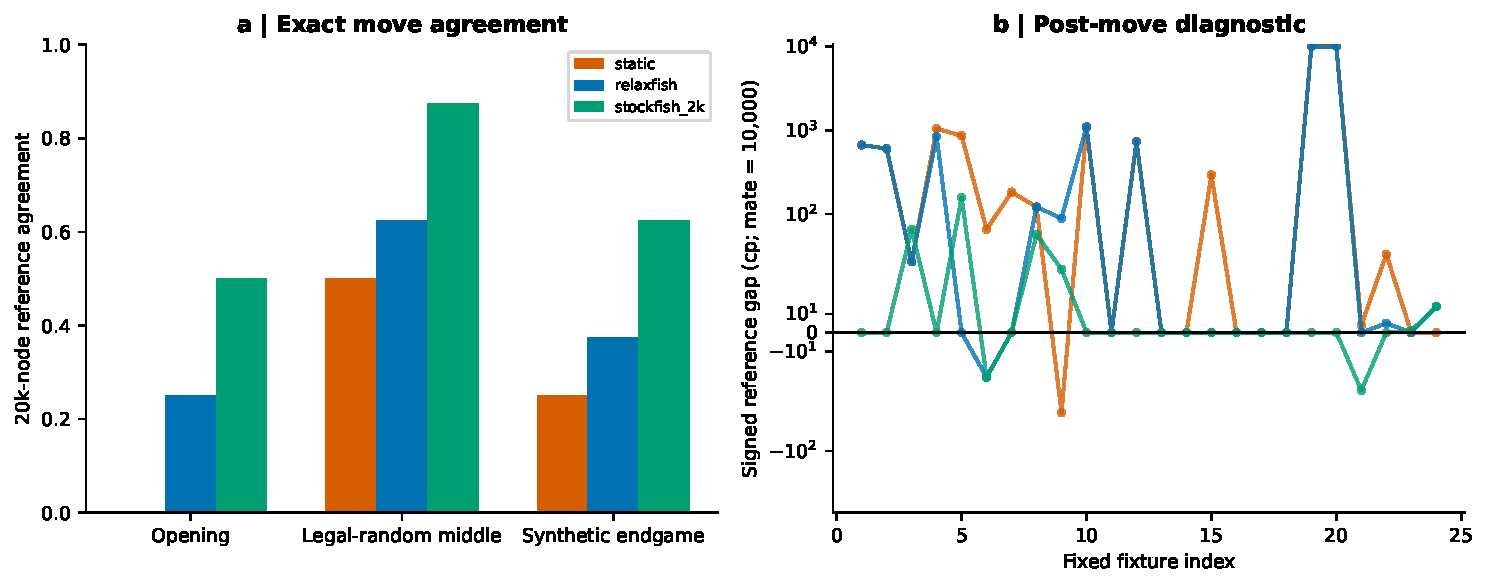
\includegraphics[width=.97\linewidth,height=.35\textheight,keepaspectratio]{figures/reference_comparison.pdf}\end{center}
{\small\textcolor{ink}{Figure 3. Diagnostic comparison against versioned Stockfish. Left, exact move agreement by fixture category, with eight positions per category. Right, signed post-move reference gaps for all positions. The symmetric logarithmic axis accommodates mapped mate scores; the gap is a noisy comparator diagnostic, not certified regret.}\par}\end{minipage}

\clearpage
\section*{10. The opponent gets a vote}
The four diagnostic games all ended in checkmate losses for Relaxfish. After the shared Italian opening, the White-side prototype survived 86 additional plies and the Black-side prototype 45. After the Queen's Gambit opening, the corresponding continuations lasted 34 and 39 plies. The released move sequences permit each result to be replayed.

These losses do not answer the proposed architecture's final strength. They answer a narrower question about the current implementation: one-ply relational evaluation is not enough to withstand the tested Stockfish search. That is a useful and concrete answer. It identifies a horizon problem that further role concentration alone cannot repair.

There is no benefit in rewriting a checkmate as a near-success. The programme's ambition survives because it is attached to an engineering and mathematical proposal, not to a fabricated score. The next implementation must improve tactical depth, preserve defensive alternatives and measure whether relational ordering increases effective search strength at fixed resources.

This distinction also protects the title from becoming a substitute for evidence. Better Than Stockfish'' is the standard I intend to meet. In this article, the prototype establishes an executable foothold, a transparent ablation and a protocol capable of rejecting premature victory claims. The strongest voice a research article can have is one that lets the opponent refute it.

A match demonstration is not a statistically powered tournament. The openings are not randomly sampled from a declared population, the resource budgets are not equal, and there are only two independent starting positions. The paired design reveals colour dependence but provides too little diversity for a general strength conclusion.

The principal observation is structural: a role field can improve selected local decisions and still fail catastrophically over a game. That makes long-horizon adversarial response the natural next target. Relaxfish must learn not merely to name a plan, but to preserve the plan when the opponent chooses the move that is least convenient for it.

\clearpage
\section*{11. Concentration, coherence and the confidence trap}
Role distributions sharpen during the executed relaxation. The mean row entropy is

\[
H(q)=-\frac1N\sum_{i,r}q_{ir}\log q_{ir}.
\]

Low entropy means the inference assigns each piece a relatively concentrated role. High entropy means several roles retain support. Neither quantity is a direct measure of tactical accuracy. A bad position can have a very coherent losing plan.

This matters because the human interface is persuasive. A dragon queen, a named knight and a highlighted attack cluster can make the inferred plan easy to understand. They can also make an untested plan feel more certain than it is. The interface should therefore expose two distinct objects: role confidence and search evidence.

The potential trajectories establish the implemented update's behaviour on the released states. The entropy trajectories describe concentration. The four match losses establish that concentration does not confer practical invulnerability. These results belong together rather than being separated into a flattering visualization and an inconvenient footnote.

I propose three interface readouts for a mature engine. A role readout describes what the relational model is emphasizing. A response readout shows the strongest discovered counterplay and how budgets change it. A certificate readout gives the sound interval, if one is available. The first can become sharp while the third remains broad.

For scientific use, role confidence should be calibrated against a defined target before being presented as probability. A possible target is the stability of a role under nearby legal continuations. Another is the success of a proposed plan under a response population. Neither target is identical to this move wins.'' Calibration must specify which event is being predicted and evaluate it on held-out cases.

Entropy can still guide computation. An ambiguous role assignment may indicate a useful place to spend search effort; a concentrated assignment can supply a candidate ordering. The proper test is whether such allocation improves outcomes or certificate closure at a given budget. The representation earns authority by helping the search withstand opposition.

\begin{minipage}{\linewidth}\begin{center}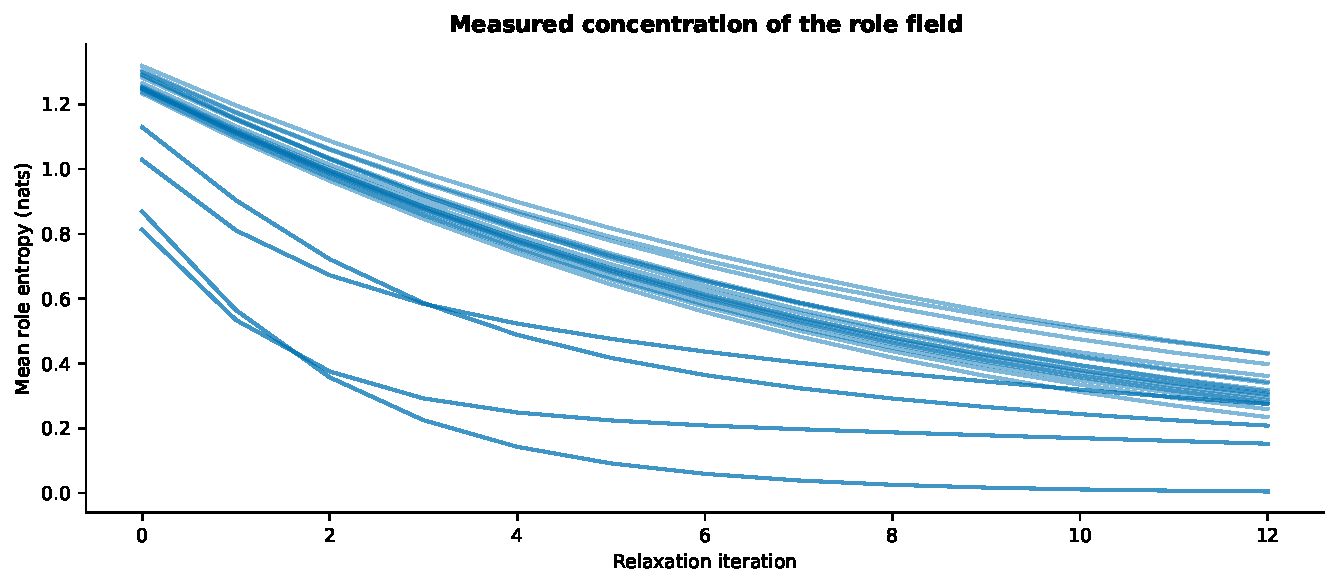
\includegraphics[width=.97\linewidth,height=.35\textheight,keepaspectratio]{figures/entropy.pdf}\end{center}
{\small\textcolor{ink}{Figure 4. Measured role entropy across twelve updates on all 24 fixtures. The ordinate is the mean Shannon entropy of piece-role rows in nats. These curves describe representation concentration. They do not estimate win probability or strategic exploitability.}\par}\end{minipage}

\clearpage
\section*{12. Exact bounds in the habitat}
Chess Critter supplies a separate test bed in which every searched node can retain an honest outcome interval. Its state includes the shared rectangle, all surviving armies, turn, movement rights, en passant, quiet-move count, repetition history and elapsed ply count. A checked king with no individual rescue retires its original army; victory requires all opposing kings to be retired. These are variant rules, not standard chess.

Unexpanded nodes receive $[-1,+1]$. Terminal nodes receive $[v,v]$, where $v$ is the exact White-perspective result under the habitat rules. If children carry sound intervals $[l_a,u_a]$, White nodes propagate

\[
[l,u]=[\max_a l_a,\max_a u_a],
\]

and Black nodes propagate $[\min_a l_a,\min_a u_a]$. These operations preserve enclosure because maximum and minimum are monotone in each argument. A budget interruption leaves unvisited alternatives at their full interval.

The solver uses iterative deepening, retains tighter root-move bounds across iterations and orders captures and promotions first. It does not replace exact leaf values with the role evaluator. Proving a White win can stop once a move's lower bound reaches +1; proving a Black win can stop once an upper bound reaches -1. A draw may require much broader exclusion of alternatives.

The automatic 1,200-ply cap supplies a finite horizon. Complete eventual expansion therefore reaches an exact result in principle, provided the rule implementation is correct and required branches are not permanently omitted. Practical convergence can be prohibitively expensive. A five-second run from the ordinary 8-by-8 initial formation examined 24,491 nodes, completed three-ply search and retained $[-1,+1]$.

Tests establish mate-in-one for both teams, stalemate, horizon draws, history preservation, unchanged live state, sound interrupted intervals and agreement with independent exhaustive two-ply searches. These are small but genuine certificates. The habitat is where the meaning of closure can be inspected before anyone attempts to pronounce standard chess solved.

\clearpage
\section*{13. The empirical game and its missing strategies}
Suppose a league contains White policies $P_W=\{\pi_W^1,\ldots,\pi_W^m\}$ and Black policies $P_B=\{\pi_B^1,\ldots,\pi_B^n\}$. The payoff matrix is $A_{ij}=u_s(\pi_W^i,\pi_B^j)$. A restricted equilibrium solves

\[
v_P=\max_{x\in\Delta^{m-1}}\min_{y\in\Delta^{n-1}}x^\top Ay.
\]

This empirical game is a well-defined object. Solving it exactly does not mean the full chess game has been solved. Its policies form a chosen subset of all policies, and an omitted strategy may exploit the restricted equilibrium.

An expanding response procedure supplies the bridge. Solve the current restricted game, search for a White response to the Black mixture and a Black response to the White mixture, add productive responses, and repeat. Research on double-oracle methods formalizes this strategy of growing the policy population [4]. Relaxfish adopts that experimental logic without claiming the present pilot implements it.

Let $\widetilde U$ and $\widetilde L$ be the strongest discovered threats and guarantees. A White maximization oracle with additive error $\rho_W$ satisfies $\widetilde U\le U\le\widetilde U+\rho_W$. A Black minimization oracle with error $\rho_B$ satisfies $\widetilde L-\rho_B\le L\le\widetilde L$. Therefore

\[
U-L\le(\widetilde U-\widetilde L)+\rho_W+\rho_B.
\]

Without valid oracle-error bounds, the discovered gap is diagnostic. It can be small while true exploitability remains large. In fact, exact payoff measurements against a restricted opponent set usually give lower bounds on the available exploitability: the strongest discovered attack is no stronger than the strongest possible attack.

The league's value is that new attacks can become permanent experimental objects. Each discovered counterexample expands the population and challenges subsequent releases. Empirical progress becomes the increasing ability to survive known attacks and the decreasing success of new response searches. The universal claim requires the additional oracle and coverage argument; the empirical claim requires those limits to be stated rather than hidden.

\clearpage
\section*{14. Draws, repetition and the stalemate gambit}
A draw is a terminal result. A forced draw is a strategic guarantee. Threefold repetition along one observed line supplies the former immediately and the latter only after relevant alternatives have been resolved. The distinction is exactly the issue that motivated this programme.

The habitat's forage policy is a seeded local heuristic. It can steer into a loop even when a winning alternative exists. Material dominance, spatial occupation and a visually coherent attack can all coexist with a repetition draw. The stronger player may have failed to maintain progress; the defender may have found genuine perpetual counterplay; both policies may simply prefer the same cycle.

To investigate a forced draw, begin from a state before the decisive repetition and include its history. Ask whether the defending side has a strategy that prevents defeat against every attacking continuation. To investigate a forced repetition specifically, require the stronger condition that its strategy forces the repetition outcome rather than another kind of draw. These are different search objectives.

The stalemate gambit is a legitimate adversarial idea: give the opponent an opportunity to acquire material while preserving a drawing resource. Its success depends on reachable legal configurations, not on the rhetorical power of the word gambit. In a losing position, a forced draw is an improvement; in a winning position, voluntarily accepting one can abandon the win.

A practical Relaxfish response suite should include perpetual checks, fortress-like blockades, underpromotions, sacrifice-to-stalemate mechanisms and repetition escapes. The opponent class must include policies that deliberately search for these resources rather than merely maximize conventional material scores. Otherwise the evaluation can flatter an attacker by never supplying the defence that refutes it.

This is also why draw frequency cannot be the sole objective. A programme that repeats harmlessly may draw often while being strategically brittle elsewhere. The desired object is a robust policy whose drawing or winning guarantee survives adversarial choice. The observed terminal label is the beginning of that investigation, not its final mathematical explanation.

\clearpage
\section*{15. Statistical significance with a declared population}
I take statistical evidence seriously. The relevant question is which random quantity the experiment estimates. Let $X\in[0,1]$ be Relaxfish's match score against a frozen testing distribution, with win 1, draw 1/2 and loss 0. The sample mean estimates $\mu=\mathbb E[X]$. It does not directly estimate the minimax value of chess.

For independent bounded trials, a standard concentration bound gives

\[
\Pr(|\widehat\mu-\mu|>e)\le2\exp(-2ne^2).
\]

Solving for $e$ yields $e=\sqrt{\log(2/\delta)/(2n)}$ for confidence at least $1-\delta$. The utility scale, confidence level and sample size are explicit. The bound is conservative and says nothing about challenges absent from the testing distribution.

Opening pairs are the natural independent units when colours are swapped from a common starting state. If $X_{i,W}$ and $X_{i,B}$ share opening $i$, define $Y_i=(X_{i,W}+X_{i,B})/2$. Concentration can apply to independent pairs $Y_i\in[0,1]$. Treating correlated games as twice as many independent observations understates uncertainty.

A test of superiority and a test of equivalence ask different questions. Rejecting no advantage'' supports a positive performance difference under the protocol. Establishing closeness to a draw requires an equivalence margin specified before evaluation and an interval contained within that margin. Failure to reject a win advantage is not affirmative evidence of equivalence.

Repeated deterministic self-play from the same state is not an independent sample of hidden strategic alternatives. It can be a reproducibility check. Random openings, randomized policies or independent response seeds can supply sampling variation, but their distribution must be declared. The statistical analysis describes that distribution rather than a universal adversary.

The protocol therefore freezes evaluation populations and separates exploratory tuning from confirmatory matches. A small sigma is useful when it belongs to an interpretable estimator. The aim is to make that estimator answer the scientific question we actually intended to ask.

\clearpage
\section*{16. Zero failures and the confidence surface}
Suppose a frozen challenge distribution produces an exploitable failure with probability $p$. If $n$ independent challenges produce zero failures, then $\Pr(K=0)=(1-p)^n$. Inverting this expression gives the exact one-sided bound

\[
p_{\rm upper}=1-\delta^{1/n}.
\]

The interpretation is precise: at fixed sample size, a procedure that reports this upper limit after zero failures has its declared coverage under the Bernoulli model. It is an upper bound on failure frequency under the challenge distribution. It is not an upper bound on the utility of the strongest possible untested strategy.

At confidence 95 percent, approximately 299 independent zero-failure challenges are required to put the upper failure frequency below 0.01. Roughly 29,956 are required for 0.0001. Making the target microscopic demands an enormous number of independent trials. A tolerance near $10^{-64}$ cannot be established by a plausible match count using this route.

That calculation is not a dismissal of empirical solving. It explains where mathematical structure becomes indispensable. Exact subgame certificates, demonstrably adequate response oracles and carefully justified coverage arguments can answer questions that random challenges alone cannot efficiently settle. Statistical evidence and structural reasoning should cooperate.

The figures on this page plot the formula itself. They are analytic design calculations, not reported Relaxfish results. Their colour encodes the bound; the axes encode sample count and confidence. They provide a practical planning tool for choosing a scientifically meaningful tolerance before resources are committed.

Adaptive stopping changes the analysis. A researcher who checks the interval after every new batch and stops when it looks favourable cannot reuse a fixed-sample guarantee without adjustment. A predeclared stopping rule or an appropriate anytime-valid procedure is required. Sequential analysis is part of the protocol rather than a licence to stop at the prettiest number.

\begin{minipage}{\linewidth}\begin{center}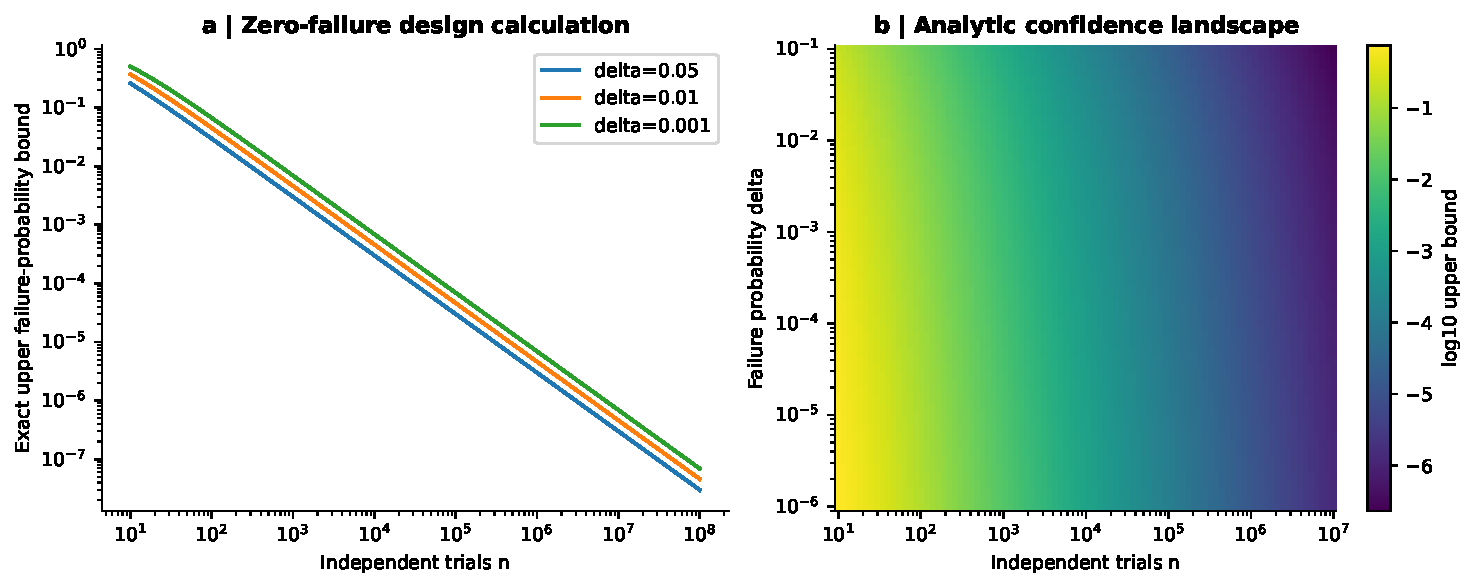
\includegraphics[width=.97\linewidth,height=.35\textheight,keepaspectratio]{figures/statistical_design.pdf}\end{center}
{\small\textcolor{ink}{Figure 5. Analytic fixed-sample design calculations. Left, exact one-sided failure-frequency bounds after zero observed failures. Right, the same expression as a colour map across sample count and confidence parameter. These curves assume independent Bernoulli challenges and are not engine-performance measurements.}\par}\end{minipage}

\clearpage
\section*{17. A three-dimensional view of uncertainty}
The confidence landscape is a surface in sample size, confidence demand and upper failure-frequency bound. Its shape makes an important practical fact visible: stronger confidence and smaller target error both cost observations. The effect is smooth on logarithmic axes and severe at extreme targets.

The surface is generated from $\log_{10}(1-\delta^{1/n})$, using numerically stable arithmetic. For large $n$, cancellation can corrupt direct subtraction. The released implementation evaluates $-\operatorname{expm1}(\log\delta/n)$, which retains small differences more reliably. Numerical accuracy supports the design calculation; it does not manufacture additional statistical evidence.

This is one place where epsilon and sigma genuinely meet. Sigma summarizes variation under a stochastic sampling model. Epsilon specifies an acceptable error in the target quantity. A confidence calculation connects them only after the model, estimator and target are fixed. That connection is powerful, and it should be written rather than assumed.

The same three-dimensional visual grammar can display future adversarial experiments: budget on one axis, opponent diversity on another, and discovered exploitability on the third. Such a plot would need measured data at each grid point, a declared treatment of missing runs and uncertainty bars. The present article does not substitute a hypothetical surface for those future measurements.

A mature research dashboard should distinguish measured surfaces, analytic surfaces and architectural diagrams. The distinction belongs in titles and captions because readers often see figures before reading the methods. The figures here are colour coordinated but epistemically explicit: analytic confidence plots show a theorem-based design expression; measured role plots show executed calculations.

My aim is not to reduce the programme's ambition to a timid error bar. It is to make the ambition traversable. A surface that exposes the cost of a claim tells us where a better theorem, a stronger response search or a more efficient implementation would actually change the feasibility of the project.

\begin{minipage}{\linewidth}\begin{center}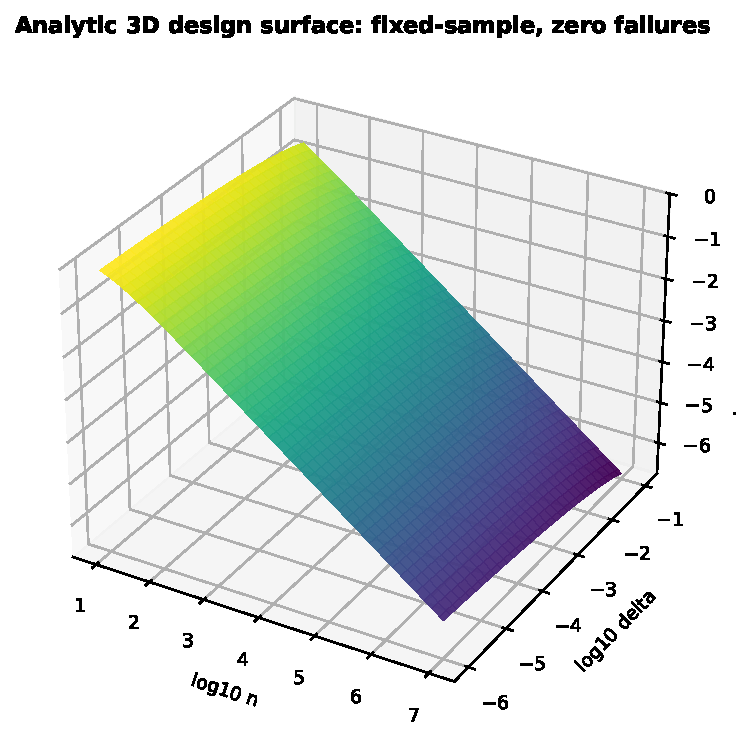
\includegraphics[width=.97\linewidth,height=.35\textheight,keepaspectratio]{figures/confidence_3d.pdf}\end{center}
{\small\textcolor{ink}{Figure 6. Three-dimensional analytic confidence surface. The horizontal coordinates are log10 independent challenge count and log10 confidence parameter; height is log10 of the exact zero-failure upper bound. This is a mathematical design surface, not an extrapolated claim about Relaxfish.}\par}\end{minipage}

\clearpage
\section*{18. The landscape inside the relational model}
The compatibility potential can also be inspected geometrically. Fix a position and all role rows except one. On the selected piece's row, vary attacker weight $a$ and defender weight $d$ subject to $a\ge0$, $d\ge0$ and $a+d\le1$. Distribute the remaining mass across the other five roles in their original proportions.

This creates a triangular slice of the product-simplex domain. The released three-dimensional plot uses the Sicilian fixture and the piece on e4. Its height is the actual implemented potential with all unary, pair and triple terms recomputed on the slice. The plot contains no fitted landscape and no invented trajectory.

Because every factor in this prototype is multilinear in distinct piece rows, fixing all other rows leaves an affine dependence on the selected row. The slice therefore forms a planar patch. This is a useful diagnostic: a curved surface in this particular calculation would suggest that a term, index or normalization had changed. Nonconvexity belongs to the joint multi-row optimization, not to this one-row slice.

Higher-order structure remains important even when a one-row slice is affine. A triple term couples three independent coordinates. Varying them together produces products and nontrivial joint geometry. The importance of the term is an empirical question: it may identify coordinated attacks, add negligible information or exaggerate a vulnerable attacking plan.

An ablation should therefore compare unary-only, unary-plus-pair and unary-plus-pair-plus-triple fields at equal time. The present pilot compares the full role contribution with its removal. It does not isolate the triple term's marginal contribution. That narrower experiment is part of the prospective next study.

The purpose of a landscape figure is to make the computational object inspectable. It gives a reader a way to see how a representation responds to a change, but it does not transform compatibility into strategic truth. The opponent still determines whether the corresponding move survives.

\begin{minipage}{\linewidth}\begin{center}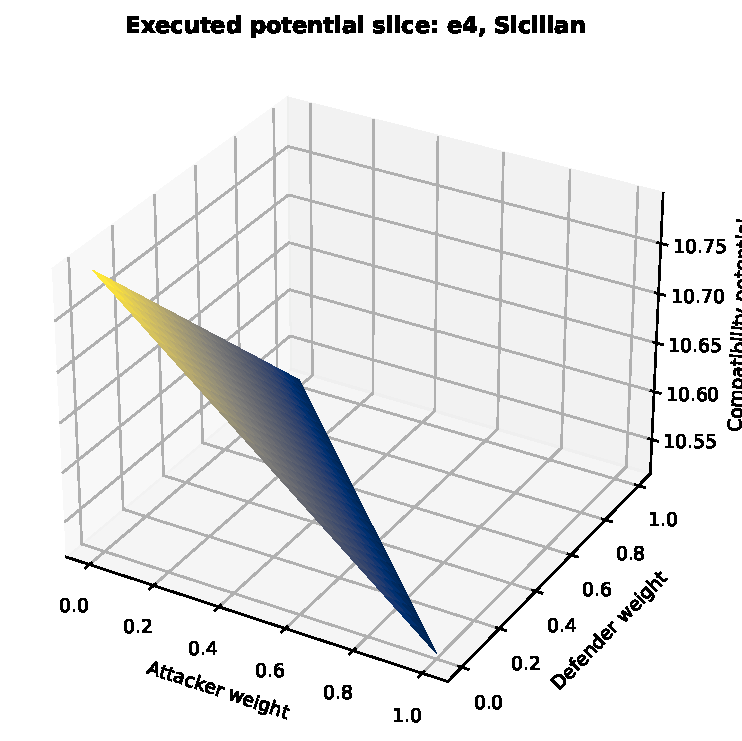
\includegraphics[width=.97\linewidth,height=.35\textheight,keepaspectratio]{figures/potential_3d.pdf}\end{center}
{\small\textcolor{ink}{Figure 7. Three-dimensional slice of the executed compatibility potential. Attacker and defender weights vary for the e4 piece in the Sicilian fixture, with remaining mass distributed proportionally across other roles and all other piece rows fixed. The triangular domain enforces normalization. The affine patch follows from multilinearity in distinct piece rows.}\par}\end{minipage}

\clearpage
\section*{19. Compute is part of the scientific claim}
An engine does not receive infinite time at the board. The cost of inference is therefore part of the hypothesis. If role relaxation consumes the same time as a useful additional search layer, it must provide a benefit that deeper search alone does not.

The observed median timing ratio of 3.88 is a warning about the current implementation, not a verdict on the architecture. The pilot uses Python, reconstructs geometric features at each evaluated successor and performs dense small-matrix operations. Stockfish is a mature optimized engine. Comparing their raw speeds at different node definitions cannot isolate the value of relaxation.

A fair strength experiment equalizes wall time or a clearly justified resource measure. A scientific ablation also equalizes the search framework. The desired comparison is the same move generator, same terminal rules, same search enhancements and same time control, with the relational component toggled. Hash size, threads, warm-up, processor affinity and batch ordering should be fixed or randomized as specified.

Potential optimizations include incremental attack maintenance, sparse coalition storage, cached role features and selective re-inference after a move changes the relevant neighbourhood. These optimizations can alter numerical output and must be checked against the baseline implementation. Speed gained by silently changing the mathematical model is a separate treatment, not an exact acceleration.

Move ordering offers a particularly clean integration point. A role model can suggest which legal alternatives to search first while leaving the set of alternatives intact. A correct alpha-beta search can then return the same fixed-depth result with fewer visited nodes, depending on ordering quality. Under a time budget, that saving may enable greater depth.

The engineering question is concrete: does the model improve the strength-versus-time curve? The plot on this page measures the pilot's current cost and its paired diagnostic changes. Future curves require repeated timings and match outcomes at multiple budgets. The claim better'' must eventually live on those curves.

\begin{minipage}{\linewidth}\begin{center}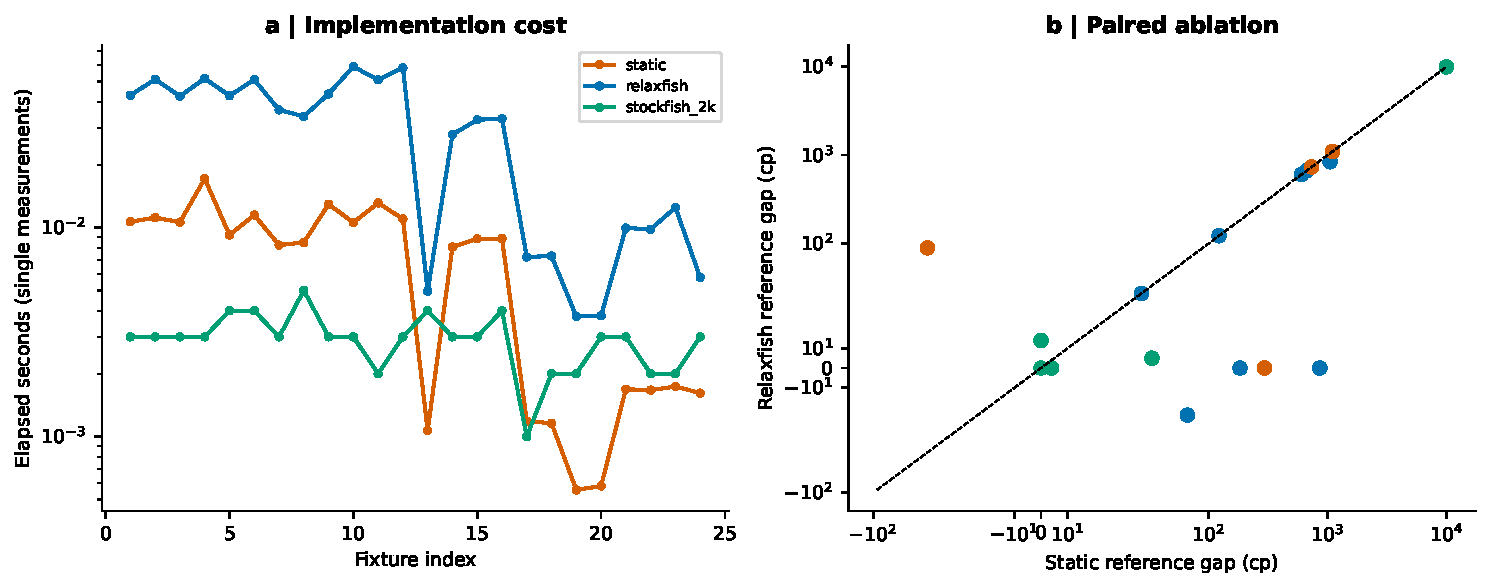
\includegraphics[width=.97\linewidth,height=.35\textheight,keepaspectratio]{figures/ablation_cost.pdf}\end{center}
{\small\textcolor{ink}{Figure 8. Decision cost and paired diagnostic changes. Left, single elapsed-time measurements per fixture for the two Python choosers and Stockfish's reported 2,000-node analysis time. Right, static versus Relaxfish signed reference gaps, with colour identifying fixture category. Different node definitions and implementations prevent a fair strength ranking from these timings.}\par}\end{minipage}

\clearpage
\section*{20. The prospective superiority protocol}
The next confirmatory experiment freezes a Relaxfish version and tests it against a named current Stockfish binary. The official release page identifies Stockfish 19, released on 5 September 2026 [2]. The executed pilot uses the older installed 14.1 binary. Those are different opponents, and the eventual title claim must identify which one has been defeated.

A serious comparison uses balanced opening pairs, equal time controls, a declared opening population and a development holdout. White and Black swap the same opening. The evaluation unit is the pair. Engine crashes, illegal moves, time losses and censored runs receive predeclared treatment rather than post-hoc reinterpretation.

The primary endpoint is paired mean score. The superiority threshold and error probabilities are fixed before the confirmatory run. If sequential testing is chosen, the likelihood model and stopping boundaries are specified in advance. Stockfish's own testing documentation describes paired outcome modelling and sequential tests [3]; Relaxfish should meet at least that level of experimental seriousness without pretending this pilot already does.

A minimum useful campaign includes several time controls and independent engine families. A short-time gain can disappear at longer budgets; a gain against one architecture can fail against another. The results should report score, uncertainty, resource use and sensitivity by opponent rather than compress every result into one attractive Elo number.

The benchmark article must include negative controls. Random legal play, material-only evaluation, role inference without pair terms and role inference without triple terms help identify where gains arise. A conventional search-only improvement tests whether the relational mechanism adds information or merely benefits from unrelated engine development.

The confirmatory criterion is deliberately demanding: a confidence interval exceeding the superiority margin under the frozen protocol, followed by replication on held-out openings and an independent budget condition. Meeting that criterion would justify better than the tested Stockfish release under these conditions.'' A broader claim would require broader evidence.

The title is therefore a research destination with a route map. It is neither a claim that four losing games were victories nor a promise that no future opponent could surpass the engine.

\clearpage
\section*{21. The prospective approximate-solving protocol}
After superiority testing, the programme changes its endpoint. The question becomes whether increasingly diverse and increasingly well-funded response searches can exploit the candidate policies. A draw-rich league alone is insufficient; the experiment must actively seek departures from its apparent equilibrium.

Freeze candidate policies and a testing distribution. Build a response population containing conventional engines, independently trained neural engines, draw specialists, tactical specialists and prior counterexample policies. Each response receives declared budgets. Store the strongest discovered exploitation, not just the average league score.

Response search should escalate along several axes: search time, initialization diversity, opening distance, policy architecture and targeted mechanism. A policy that is safe against superficial responses can fail under a longer search in a single narrow endgame. Stratified reporting keeps that failure visible.

For each candidate pair, report empirical response gaps with uncertainty, explicit oracle assumptions and coverage limitations. If response oracles have proven additive errors, combine them with payoff estimation bounds. If they do not, label the gap as discovered exploitability and avoid presenting it as an upper bound on all possible exploitation.

This document specifies future testing and is not an external preregistration. The stopping criterion requires a declared tolerance $\epsilon$ in utility units and confidence $1-\delta$. A valid certificate may combine exact subgame results with statistical bounds on a declared challenge distribution. The bridge from distributional protection to universal protection must be separately justified. A coverage assumption is a substantive hypothesis about omitted strategies, not a cosmetic term in the notation.

The full starting position is only one state, but a practical policy acts in many reachable states. Reporting start-state performance and reachable-state robustness separately prevents a favourable opening distribution from concealing catastrophic off-path behaviour. Adversarially selected continuations are therefore part of the response suite.

The programme succeeds empirically when attacks become harder to find under clearly expanding tests. It succeeds mathematically when valid upper bounds close. These are compatible aspirations, and the methodology gives each a measurable meaning.

\clearpage
\section*{22. Reproducibility and implementation record}
The computational environment uses Python 3.10.12, python-chess core version 1.10.0, NumPy 1.26.4, SciPy 1.15.3 and Matplotlib 3.10.8 on a Linux machine with an Intel Core i7-1255U processor. The numerical linear-algebra thread count is set to one. Exact recorded platform and Python strings appear in the result manifest.

The benchmark script constructs the fixtures, executes all choices and comparator analyses, records the relational fields, and plays the four diagnostic games. The plot script reads those records and constructs all measured plots. It also generates the explicitly labelled analytic confidence surfaces. The verification script checks legal states and selected moves, normalized role rows, monotonic potential within tolerance, unchanged boards after search, and finite-difference agreement with the analytic gradient.

The standard-board prototype and the habitat solver are released separately in the reproduction bundle. The latter's Node tests include classic initial-position move counts of 20, 400 and 8,902, rule edge cases, multi-king adjudication and solver interruption. The manuscript does not claim that tests are a formal proof of the entire software stack. They define a useful and repeatable level of implementation evidence.

Repeatability has several layers. The fixture generator and Python move chooser are deterministic under the recorded environment and ordering. Stockfish's fixed-node searches are more controlled with one thread and a cleared hash, but compiler, platform and version can still change outputs. Timing measurements naturally vary with machine load and thermal state.

Reproduction commands are supplied in the README. Every figure is exported as a high-resolution PNG and a vector PDF. The article is available as PDF, LaTeX source and plain text, with JSON and CSV data. A SHA-256 inventory permits readers to identify the exact released artifacts.

The objective is to make disagreement productive. A reader who finds a counterexample, a numerical discrepancy or a stronger move should be able to point to a specific state and procedure. That is the practical form of reality's veto: a result can be replayed, challenged and improved.

\clearpage
\section*{23. Discussion: pruning and planting}
Mathematics prunes a claim until its assumptions and consequences are visible. Experiment plants the surviving structure in a world that can resist it. Relaxfish needs both. A beautiful compatibility field without adversarial strength is incomplete; a high match score without a clear target leaves the meaning of solution'' unsettled.

The pilot supports a modest but concrete mechanism: a relational role field changes decisions and improves selected comparator diagnostics on a fixed suite. It also supplies a decisive operational failure: shallow search loses every demonstration game. Those facts identify a focused next step, the integration of relational ordering into stronger search with equal-time evaluation.

The formal analysis supplies a second contribution. Universal strategy guarantees, response-oracle error, empirical payoff uncertainty and numerical precision are distinct objects. They can be combined only when they refer to a shared target and valid assumptions. That clarification makes an empirical approximate-solving programme stronger rather than smaller.

Several challenges remain open. Role weights may overvalue coherence; triple terms may overcount attack pressure; a manually specified evaluation may fail to generalize; colour and opening distributions may interact with the policy; and opponent populations may conceal common blind spots. Each challenge suggests a measurable ablation or adversarial test. None is resolved by raising the number of decimals in a reported score.

The proposed architecture has an advantage worth investigating: it makes tactical intent explicit at a scale that can guide attention. The engineering question is whether that intent helps the engine find the move the opponent least wants it to find. The mathematical question is whether the resulting policies can carry guarantees whose error closes under increasing computation.

I am not asking the reader to admire a claim because it is large. I am asking that the large claim be made testable. Better Than Stockfish is the first gate. Robust empirical approximate solving is the next. Exact closure is the strongest endpoint. The programme proceeds by giving each gate an opponent, a metric and a condition for failure.

\clearpage
\section*{24. Extended methods: errors, coverage and logical limits}
\textbf{Proposition 3: sound interval propagation.} Suppose every child interval contains its true value. Monotonicity of maximum or minimum gives a parent interval containing the parent's true value. Induction from exact terminals proves soundness for the explored tree, with unresolved leaves represented by $[-1,+1]$. Retaining intersections with earlier sound intervals preserves soundness. This proposition assumes complete legal alternatives and correct state transitions.

\textbf{Proposition 4: finite-horizon closure.} In a finitely branching game with a finite remaining horizon, a search that eventually expands every required branch to termination obtains the exact starting value. Proof is induction on remaining horizon. Selective ordering changes time to discovery; permanently discarding a required unresolved branch can invalidate closure. The habitat's cap supplies the hypothesis, although its exact value may differ from uncapped chess.

\textbf{Proposition 5: restricted attacks understate available exploitation.} If $P_B\subseteq\Pi_B$, then $\min_{\pi_B\in P_B}u(\pi_W,\pi_B)\ge\inf_{\pi_B\in\Pi_B}u(\pi_W,\pi_B)$. The restricted opponent makes the guarantee look at least as favourable. The analogous restricted White maximization is at most the full maximum. Thus a small discovered response gap is not automatically a small universal gap.

A minimal counterexample makes the issue plain. Two tested policies always choose paths ending in a draw. An untested White policy selects a different branch that wins against every Black response. All observed games remain draws while the full game value is +1. An engine league can therefore be completely accurate about its own payoff matrix and incomplete about the full game.

The example does not erase empirical evidence. It identifies the coverage argument the stronger claim requires. A response oracle with proven error, an exact remaining subgame or a justified strategy-covering construction can supply the missing link. Mere repetition of the same restricted contest cannot.

The logical limit is productive: a research article can claim empirical adequacy with declared assumptions, exact results in tractable subgames, and a programme for enlarging coverage. It should say exactly which of those objects has been achieved. The point is to make increasingly strong statements true.

\clearpage
\section*{25. Extended data tables}
\begin{center}\small
\begin{tabular}{lrrr}\toprule
Model & Agreement & Median gap (cp) & Median time (ms)\\\midrule
Static & 6/24 & 54.0 & 8.66\\
Relaxfish & 10/24 & 2.5 & 33.62\\
Stockfish 14.1 / 2k & 16/24 & 0.0 & 3.00\\
\bottomrule\end{tabular}\end{center}


The agreement column counts exact UCI move matches with the 20,000-node reference across 24 positions. Timing medians summarize single measurements per position. Signed reference gaps compare equal-node successor analyses; mate scores use the 10,000-centipawn mapping. The arithmetic mean is sensitive to that mapping. All entries describe the executed diagnostic rather than a fair engine-strength tournament.

\begin{center}\small
\begin{tabular}{lrrr}\toprule
Opening & Relaxfish side & Continuation plies & Result\\\midrule
Italian & white & 86 & 0-1\\
Italian & black & 45 & 1-0\\
Queens-Gambit & white & 34 & 0-1\\
Queens-Gambit & black & 39 & 1-0\\
\bottomrule\end{tabular}\end{center}


Continuation lengths exclude the shared opening moves. Every diagnostic game reached checkmate before the 120-ply cap; no censored continuation was reclassified as a draw. The colour swap is useful, but two shared openings do not support a stable Elo estimate or a population-wide superiority conclusion.

\begin{center}\small
\begin{tabular}{p{.43\linewidth}p{.48\linewidth}}\toprule
Parameter & Executed value\\\midrule
Role count & 7\\
Relaxation iterations & 12\\
Unary floor & 0.02\\
Pair coefficient & 0.18\\
Triple coefficient & 0.12\\
Role scale & 18 cp\\
Search depth & 1 ply\\
Reference / successor nodes & 20,000 / 5,000\\
Comparator threads / hash & 1 / 16 MiB\\
Seed & 20261003\\
\bottomrule\end{tabular}\end{center}


The listed constants define the pilot. They were specified before collecting the reported results. The repository does not contain an optimized or trained production Relaxfish engine. Future tuning must use separate development data, and the confirmatory evaluation must freeze the selected parameters.

\begin{center}\small
\begin{tabular}{p{.43\linewidth}p{.48\linewidth}}\toprule
Claim & Status\\\midrule
Role update is executable & Measured and verified\\
Potential increases on the suite & Measured\\
Reference agreement rises 6 to 10 & Measured; exact paired p = 0.125\\
Prototype beats Stockfish & Not established; four losses\\
Habitat small-position outcomes & Certified under variant rules\\
Current Stockfish superiority & Prospective target\\
Standard chess is solved & Not established\\
\bottomrule\end{tabular}\end{center}


The claim ledger is part of the scientific result. It distinguishes executable measurements from mathematical consequences and proposed experiments. The headline target is retained without mislabelling its evidential status. The reader can inspect the programme's ambition and the prototype's current limitations on the same page.

\clearpage
\section*{26. References and author record}
1. Rosenfeld, A., Hummel, R. A. \& Zucker, S. W. Scene labeling by relaxation operations. IEEE Transactions on Systems, Man, and Cybernetics SMC-6, 420--433 (1976). \url{https://doi.org/10.1109/TSMC.1976.4309519}\par
2. Stockfish developers. Stockfish 19 (5 September 2026). Official release announcement. \url{https://stockfishchess.org/blog/2026/stockfish-19/}\par
3. Stockfish developers. Statistical Methods and Algorithms in Fishtest. Official documentation, accessed 3 October 2026. \url{https://official-stockfish.github.io/docs/fishtest-wiki/Fishtest-Mathematics.html}\par
4. McAleer, S., Lanier, J., Wang, K., Baldi, P. \& Fox, R. XDO: A Double Oracle Algorithm for Extensive-Form Games. NeurIPS (2021); arXiv:2103.06426. \url{https://arxiv.org/abs/2103.06426}\par
5. Lockhart, E. et al. Computing Approximate Equilibria in Sequential Adversarial Games by Exploitability Descent. IJCAI (2019); arXiv:1903.05614. \url{https://arxiv.org/abs/1903.05614}\par
6. Hoeffding, W. Probability inequalities for sums of bounded random variables. Journal of the American Statistical Association 58, 13--30 (1963). \url{https://doi.org/10.1080/01621459.1963.10500830}\par
7. Schaeffer, J. et al. Checkers is solved. Science 317, 1518--1522 (2007). Authors' publication archive. \url{https://webdocs.cs.ualberta.ca/~chinook/publications/solving_checkers.html}\par
8. Silver, D. et al. Mastering Chess and Shogi by Self-Play with a General Reinforcement Learning Algorithm. Preprint (2017), arXiv:1712.01815. \url{https://arxiv.org/abs/1712.01815}\par
9. FIDE. Laws of Chess taking effect from 1 January 2023. \url{https://handbook.fide.com/chapter/E012023}\par
10. Stockfish developers. Stockfish testing framework: Fishtest. \url{https://github.com/official-stockfish/fishtest}\par
11. Nature. Formatting guide and research figure guide, accessed 3 October 2026. \url{https://www.nature.com/nature/for-authors/formatting-guide} ; \url{https://research-figure-guide.nature.com/}\par
12. Glover, M. E. Chess Maestro role labeler and Chess Critter rule and solver implementations, HRL Portfolio (2026). \url{https://rmichaelglover.github.io/hrl-portfolio/maestro.html} ; \url{https://rmichaelglover.github.io/hrl-portfolio/genesis/critter/chess-life.html}\par

\subsection*{Relation to prior work}
Relaxation labeling supplies the historical language of relational ambiguity reduction [1]. Exploitability descent [5] and double-oracle methods [4] supply related approaches to policy improvement against adversarial responses; their published convergence results depend on their own algorithmic assumptions. The success of self-play systems [8] motivates demanding empirical engine tests. The solution of checkers [7] demonstrates the distinct standard of a game-theoretic solution. These precedents motivate the programme without certifying this prototype.

\subsection*{Data, software and publication status}
All newly reported measurements are generated by the accompanying experiment. This document is an independent research manuscript prepared for the author's review, not an accepted Nature publication. The visual design takes inspiration from scientific journal conventions. No university affiliation, doctoral award, peer-review outcome or engine superiority result is implied.

\subsection*{Author's closing statement}
Let it be written, and let it be tested. A theorem is a strategy with its assumptions exposed; a proof closes the alternatives it must close. An experiment gives the world its turn. Relaxfish exists to make those turns increasingly informative. Reality retains the final veto.
\end{document}
